\subsection{External interfaces requirements}

\subsubsection{User interfaces}
\paragraph{\ac{eMSP}}
The \ac{eMSP} should be accessible through an application installed on the mobile device.
The first interface shown to the user, if not already done, is the \textit{login} page where the user has to input the email and password in order to authenticate.
From the \textit{login} page there is also the possibility to go to the \textit{sign up} page where the fields for inserting the necessary information are shown.
After logging in, there are multiple tabs in the app, which are:
\begin{itemize}
    \item A satellite map of the charging stations near user's position;
    \item A personalizable ranked list based on parameters chosen by the user (distance, price, environmental friendliness\ldots).
    \item A screen for enabling/disabling suggestions from the system and for setting up the connection to the user web calendar.
\end{itemize}
By selecting a station (from the ranked list or the satellite map) the specific information about it are shown. The user can select the date and the time slot from the available ones.

A \ac{CPO} can register to the system with a special form providing Company name, password and \gls{partita IVA}. Once the \ac{CPO} is registered and logged in, he can insert/remove the \ac{API} reference to the interface of a \ac{CPMS}.

\paragraph{\ac{CPMS}}
The \ac{CPMS} works as a web application; When a \ac{CPO}maintainer logs in he has the possibility to handle all the added stations.\\
In particular he can view: the system status, the list of charging stations and their policy, the available sockets and the \ac{SoC} of batteries.\\
The \ac{CPO}maintainers can change the policy of each charging station; in particular they can:
\begin{itemize}
    \item Choose a the energy provider from a list of \acp{DSO};
    \item Choose to use only the energy stored in the batteries and, once discharged, to go into automatic mode;
    \item Choose the automatic mode, that will pick autonomously which \ac{DSO} to use, whether to use batteries and when to recharge them;
\end{itemize}

The \ac{CPO} can also view the price of his service and set the revenue percentage for a single charge.
\todo[inline]{Check with assignment document for all the functions}

\subsubsection{Hardware interfaces}
\todo[inline]{Aggiorna Requirements con spiegazione di EnergySourceStrategy}
\paragraph{\ac{eMSP}}
The user, in order to interact with the \ac{eMSP}, must have a device that is provided with a \ac{GPS} and internet connection. Thanks to this, the user can search for close charging stations, see if those are available and can book or cancel a charge.
A Bluetooth peripheral should also be available to the user when he is in the vehicle, in order to make a connection with it. Thanks to this the device can query the vehicle infos (such as average battery consumption per kilometer, estimated autonomy and \ac{SoC}) so that the system can suggest to the user when and where to charge the vehicle.

\paragraph{\ac{CPMS}}
In order to use the \ac{CPMS}, the \ac{CPO}maintainer (the only type of user of this system) should have a personal computer with internet connection available so that it's possible to see the system info and communicate changes to the system (i.e. change the energy source of a charging station or setting the new revenue for a charge).
\todo[inline]{Check that we will always set the revenue instead of the final price in order to be consistent}

\paragraph{Charging socket}
The Charging sockets should have a pad for inserting the pin that the user have to validate the charge.

\todo[inline]{Add "We assume that Charging sockets have internet connection and an appropriate interface" to the assumptions}

\subsubsection{Software interfaces}
\paragraph{\ac{eMSP}}
The \ac{eMSP} does not provide any software interface because no external software should query this system.

\todo[inline]{Add "The software utilizes payment APIs" to the assumptions}

\paragraph{\ac{CPMS}}
The \ac{CPMS} should provide to the external world interfaces for:
\begin{itemize}
    \item Book the charges in a particular time-slot (accepting also a \textit{chargeID}, a PIN in order to authorize the charge once the user gets in the station);
    \item Get information of a particular charging station (location, price of the charge, parameter of environmental friendliness, type of charges available);
    \item Get the availability state of a particular socket;
    \item Get the future availability of the sockets managed by the system;
\end{itemize}

\todo[inline]{Compara software interfaces del CPMS con sequence per scoprire tutte le interfacce}

\subsubsection{Communication interfaces}
\paragraph{\ac{eMSP}}
The \ac{eMSP} should use internet connection in order to interact with the back-end of the system, query the different \acp{CPMS} and be connected to the electronic calendar. In order to communicate with the vehicle the user device should also be provided with bluetooth so that can retrieve data from the vehicle and use that for suggesting when and where to charge the vehicle.

\paragraph{\ac{CPMS}}
The \ac{eMSP} should be provided with a local connection in order to link all the infrastructure and make it manageable by a user in the local connection.
An internet connection should also be present in order to make the system reachable by the external world; in particular it is needed for queries and external functions made by users (like booking a charge, canceling a charge, seeing what time slots are available) and in order to manage remotely the system from the \ac{CPO}maintainers.

\subsection{Functional requirements}

\begin{enumerate}[label=\textbf{R\arabic*}]
    \item The \ac{eMSP} shall allow the users to register, providing name, surname, birthday, email, password, payment method;
    \item The \ac{eMSP} shall allow the user to login with email and password;
    \item The \ac{eMSP} shall provide information about a selected station such as types of available sockets, price for the charge, location, available time slots;
    \item The \ac{eMSP} shall reserve a socket in the right charging station with for a user who booked a charge through the application;
    \item The \ac{eMSP} shall allow only one user to book a socket in a particular time slot, so no booking collisions shall occur;
    \item The \ac{eMSP} shall allow the user to pay for a booked charge;
    \item The \ac{eMSP} shall refund the user when a charge is canceled;
    \item The \ac{eMSP} shall allow the user to see nearby\footnote{This parameter may be set by the user} charging stations ordered by distance, price or environmental friendliness;
    \item The \ac{eMSP} shall be able to connect to a web calendar, retrieve information about the appointments and parse them;
    \item The \ac{eMSP} shall be able to use the information about the appointments, the charging stations and the vehicle in order to proactively suggest to the user when and where to charge the vehicle;
    \item The \ac{eMSP} shall notify the user when the charging process is finished;
    \item The \ac{eMSP} shall aggregate different \acp{CPO};
    \item The \ac{eMSP} shall allow a \ac{CPO} to register, providing name, email, password, \gls{partita IVA};
    \item the \ac{eMSP} shall allow to add to an already registered \ac{CPO} a \ac{CPMS}, providing \ac{API} reference to the \ac{CPMS};
    \item The \ac{eMSP} shall verify the correctness of the identification data for the \acp{CPO};
    \item The \ac{eMSP} shall allow the \ac{CPO} to set the wanted revenue percentage;
    \item The \ac{CPMS} shall be reachable by \acp{eMSP} in order to perform/cancel a booking, or query the system;
    \item The \ac{CPMS} shall allow the \ac{CPO}maintainer to access to the system;
    \item The \ac{CPMS} shall allow the \ac{CPO}maintainer to modify the information about their systems, such as adding/removing charging stations, set stations sources and create/remove maintainers;
    \item The \ac{CPMS} shall allow the \ac{CPO}maintainer to choose the energy source and strategy;
    \item The \ac{CPMS} shall allow the \ac{CPO}maintainer to choose manual or automatic mode;
\end{enumerate}

\todo[inline]{What if a user finishes prematurely the charge? will he be refunded by the time of charge left?}

\clearpage
\subsubsection{Use case diagrams}
\begin{figure}[!h]
    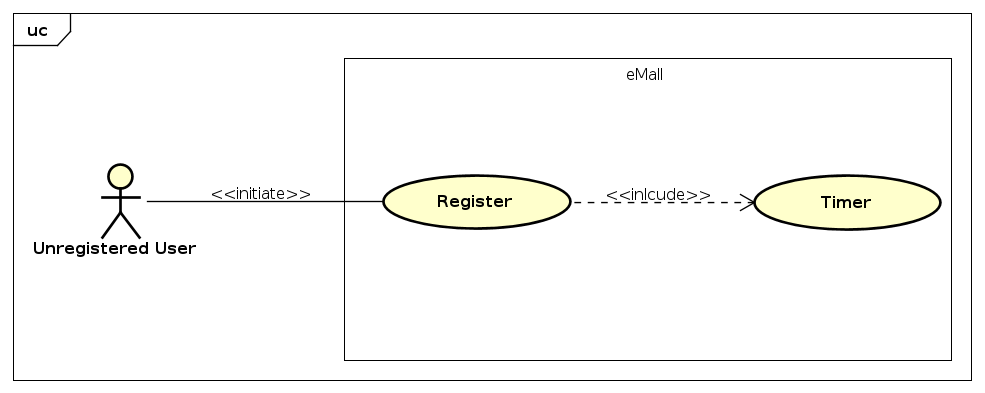
\includegraphics[keepaspectratio, width=16cm]{UseCase/UnregisteredUser.png}
    \caption{Unregistered user use case}
\end{figure}
\begin{figure}[!h]
    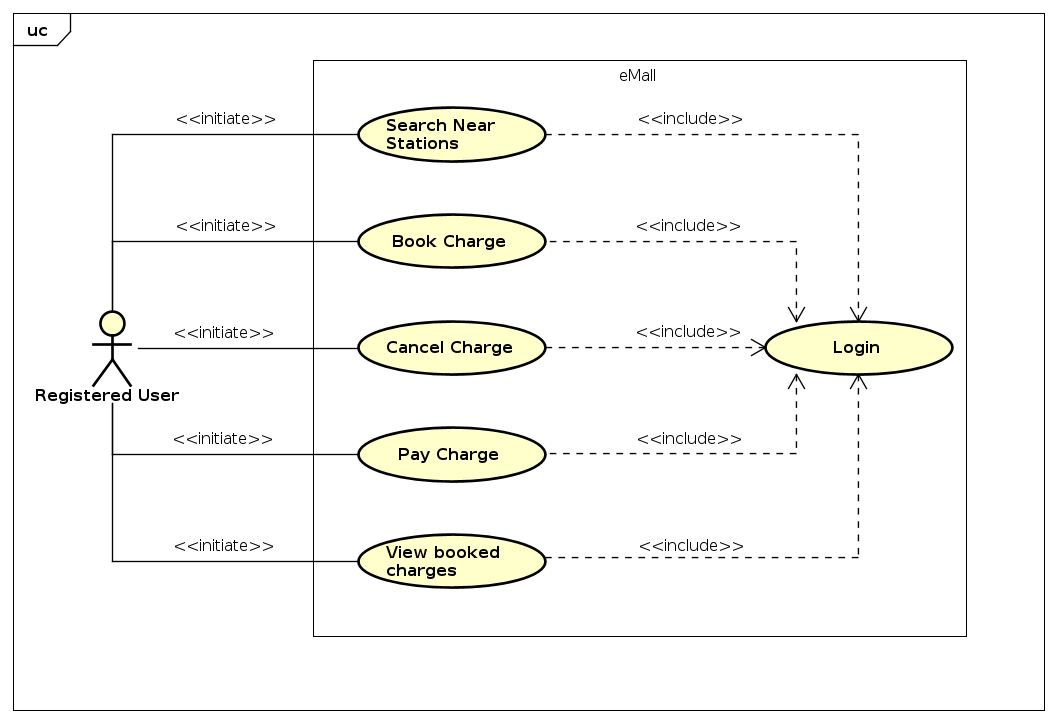
\includegraphics[keepaspectratio, width=16cm]{UseCase/RegisteredUser.png}
    \caption{Registered user use case}
\end{figure}
\begin{figure}[!h]
    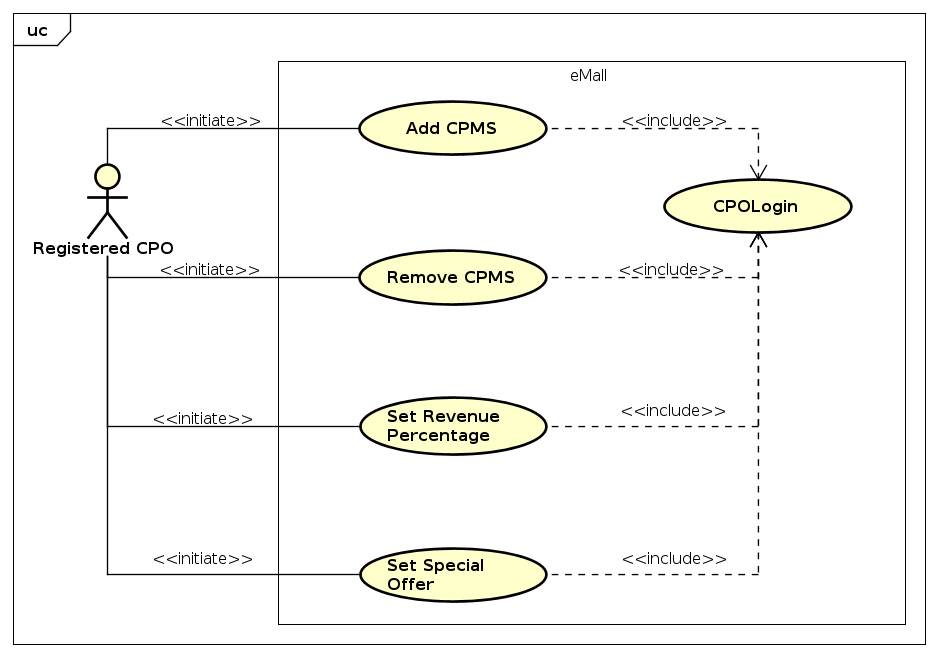
\includegraphics[keepaspectratio, width=16cm]{UseCase/RegisteredCPO.png}
    \caption{Registered \ac{CPO}}
\end{figure}
\begin{figure}[!h]
    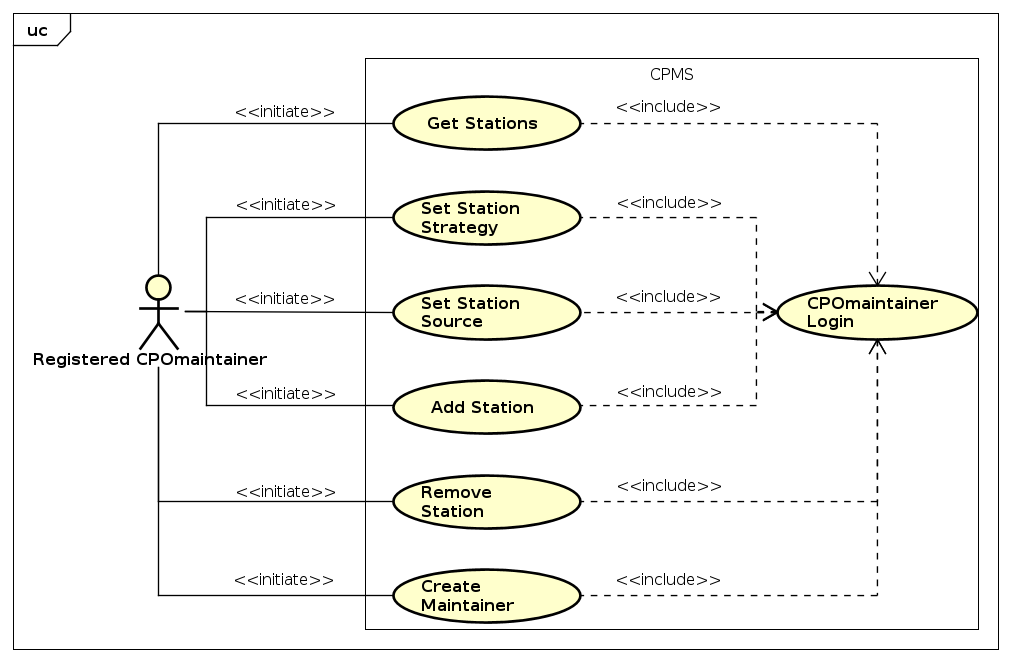
\includegraphics[keepaspectratio, width=16cm]{UseCase/RegisteredCPOmaintainer.png}
    \caption{Registered \ac{CPO}maintainer}
\end{figure}
\clearpage
\subsubsection{Sequence diagrams}
\begin{figure}[!h]
    \begin{center}
        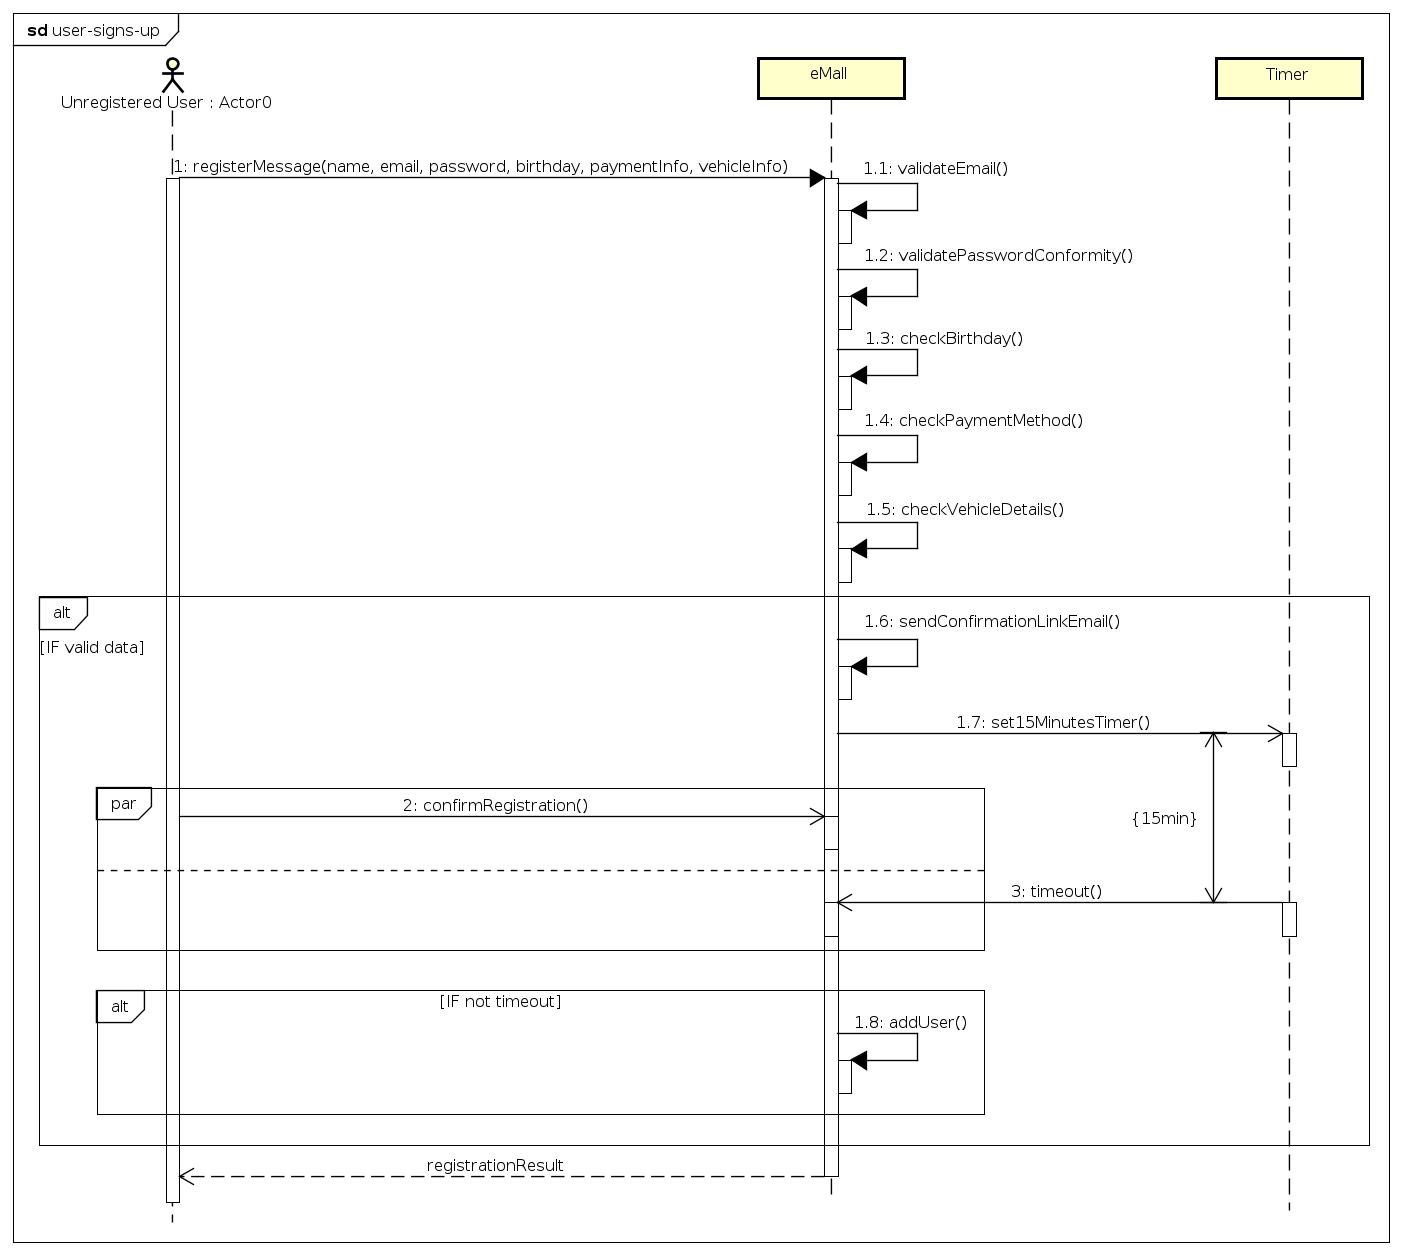
\includegraphics[keepaspectratio, width=16cm]{Sequence/user-signs-up.png}
        \caption{Registration into \ac{eMall} sequence}
    \end{center}
\end{figure}
\begin{figure}[!h]
    \begin{center}
        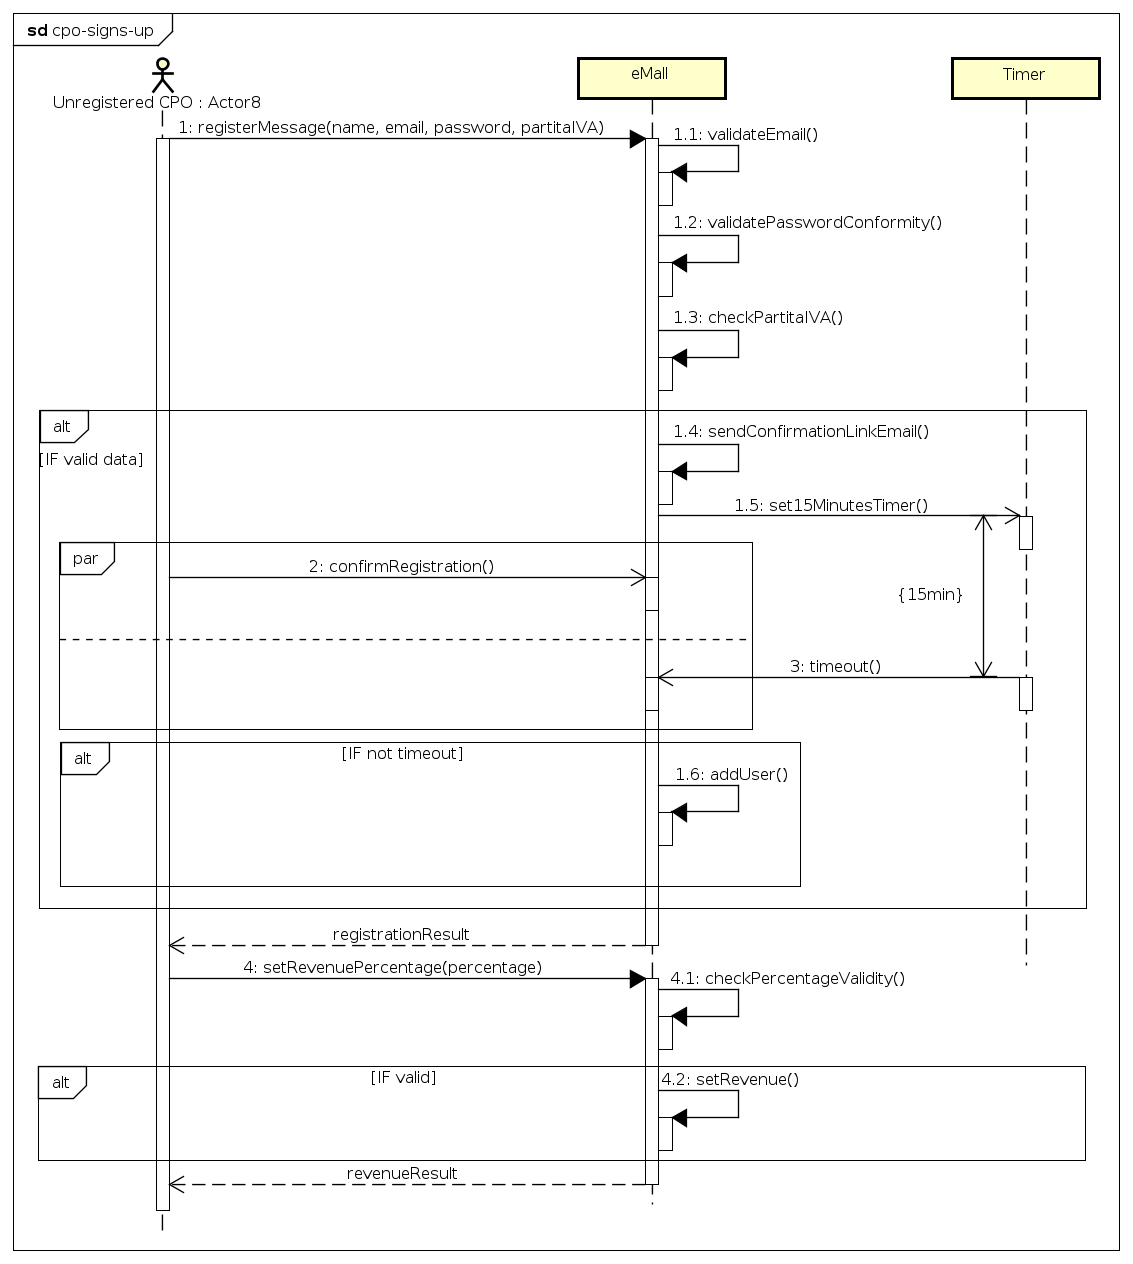
\includegraphics[keepaspectratio, width=16cm]{Sequence/cpo-signs-up.png}
        \caption{Registration of \ac{CPO} into \ac{eMall} sequence}
    \end{center}
\end{figure}
\begin{figure}[!h]
    \begin{center}
        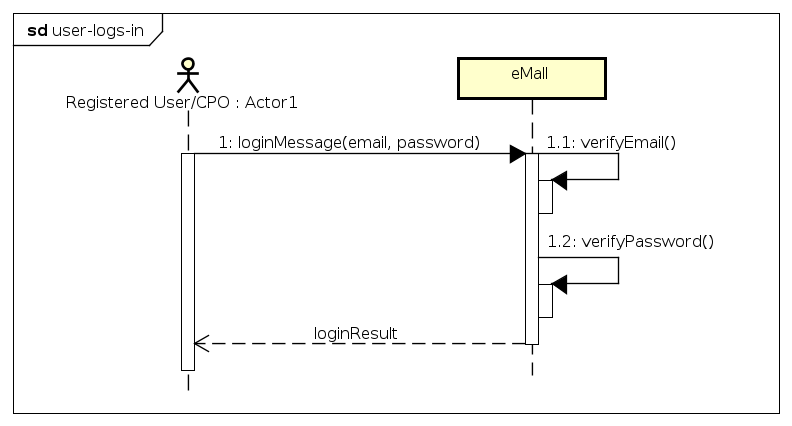
\includegraphics[keepaspectratio, width=16cm]{Sequence/user-logs-in.png}
        \caption{Login into \ac{eMall} sequence}
    \end{center}
\end{figure}
\begin{figure}[!h]
    \begin{center}
        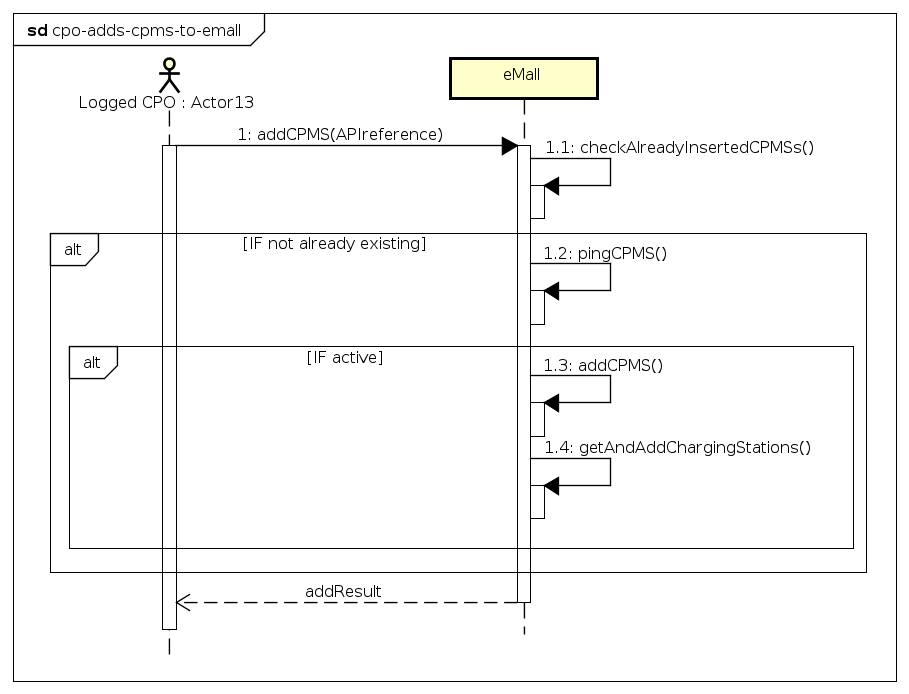
\includegraphics[keepaspectratio, width=16cm]{Sequence/cpo-adds-cpms-to-emall.png}
        \caption{\ac{CPO} adds a \ac{CPMS} into eMall}
    \end{center}
\end{figure}
\begin{figure}[!h]
    \begin{center}
        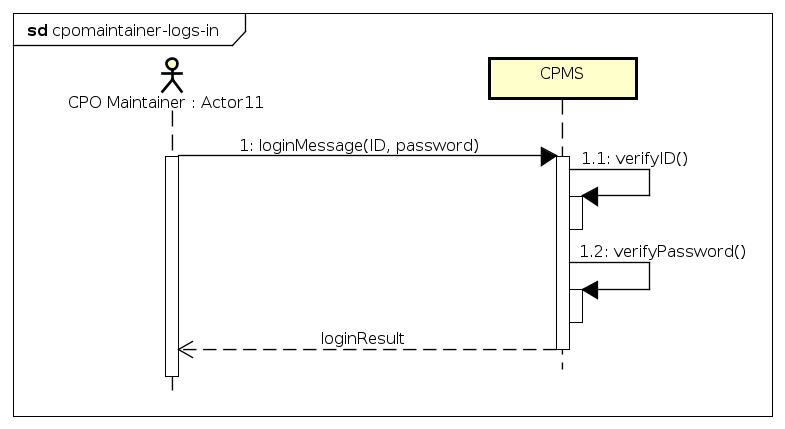
\includegraphics[keepaspectratio, width=16cm]{Sequence/cpomaintainer-logs-in.png}
        \caption{\ac{CPO} maintainer logs into \ac{CPMS}}
    \end{center}
\end{figure}
\begin{figure}[!h]
    \begin{center}
        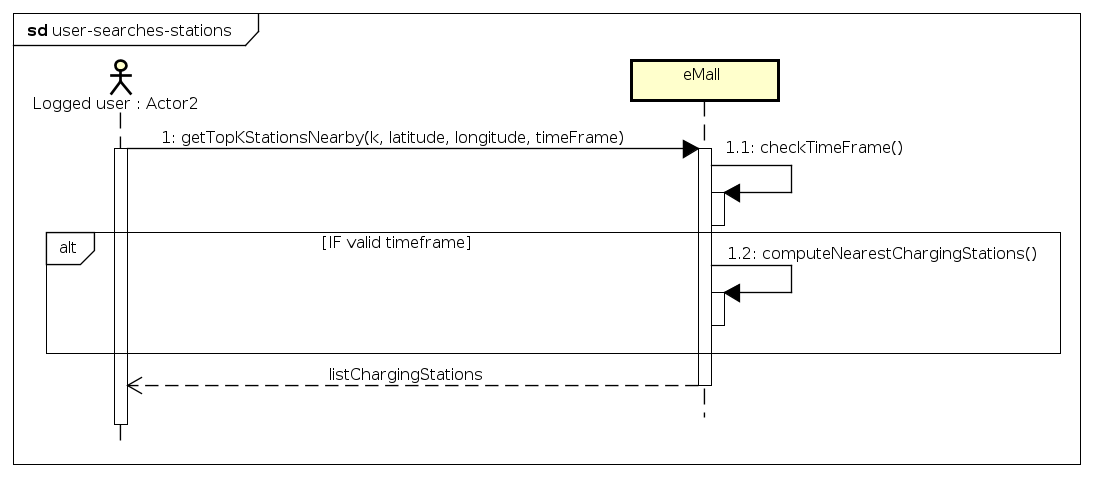
\includegraphics[keepaspectratio, width=16cm]{Sequence/user-searches-stations.png}
        \caption{Get the nearby charging stations}
    \end{center}
\end{figure}
\begin{figure}[!h]
    \begin{center}
        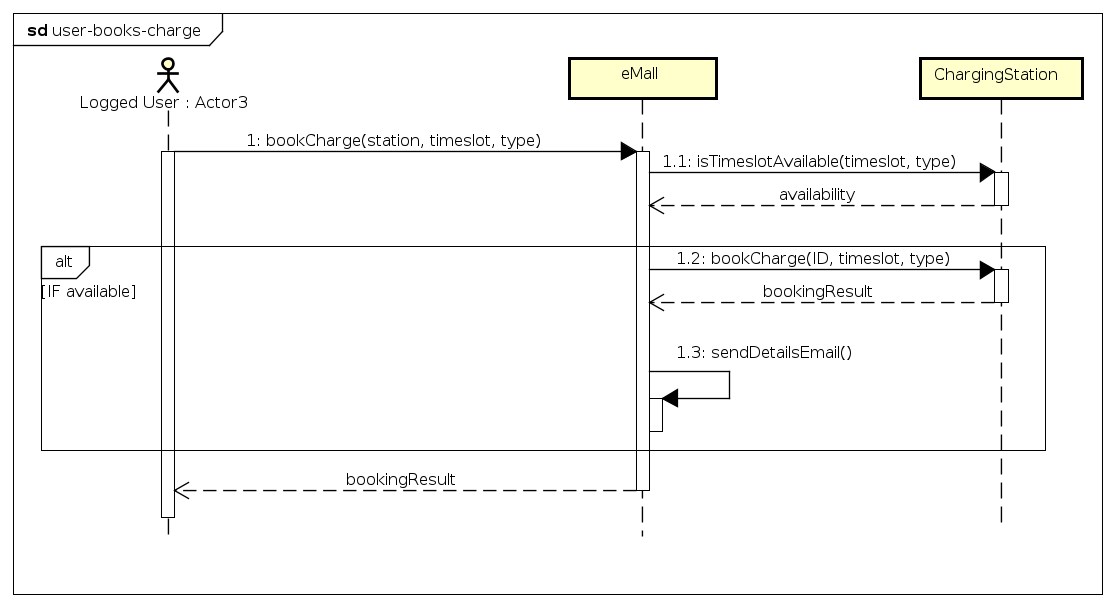
\includegraphics[keepaspectratio, width=16cm]{Sequence/user-books-charge.png}
        \caption{Book a charge sequence}
    \end{center}
\end{figure}
\begin{figure}[!h]
    \begin{center}
        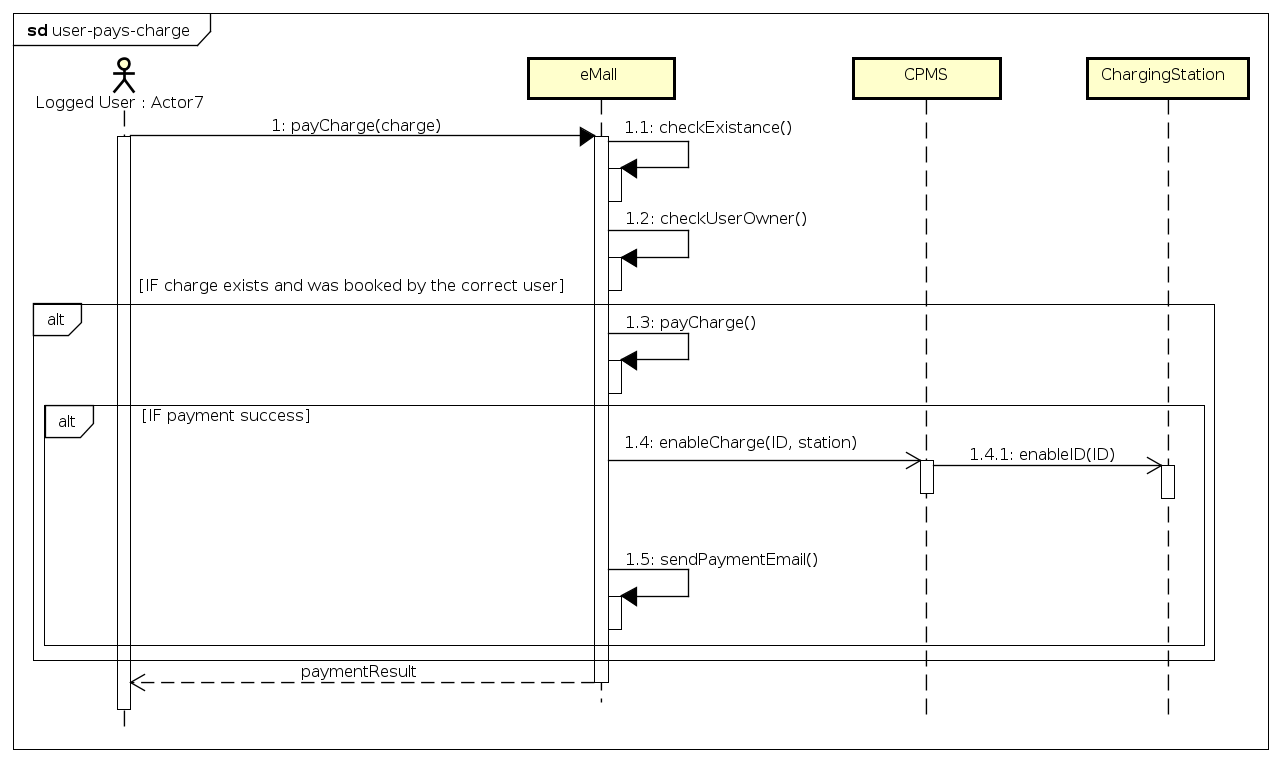
\includegraphics[keepaspectratio, width=16cm]{Sequence/user-pays-charge.png}
        \caption{Pay a charge sequence}
    \end{center}
\end{figure}
\begin{figure}[!h]
    \begin{center}
        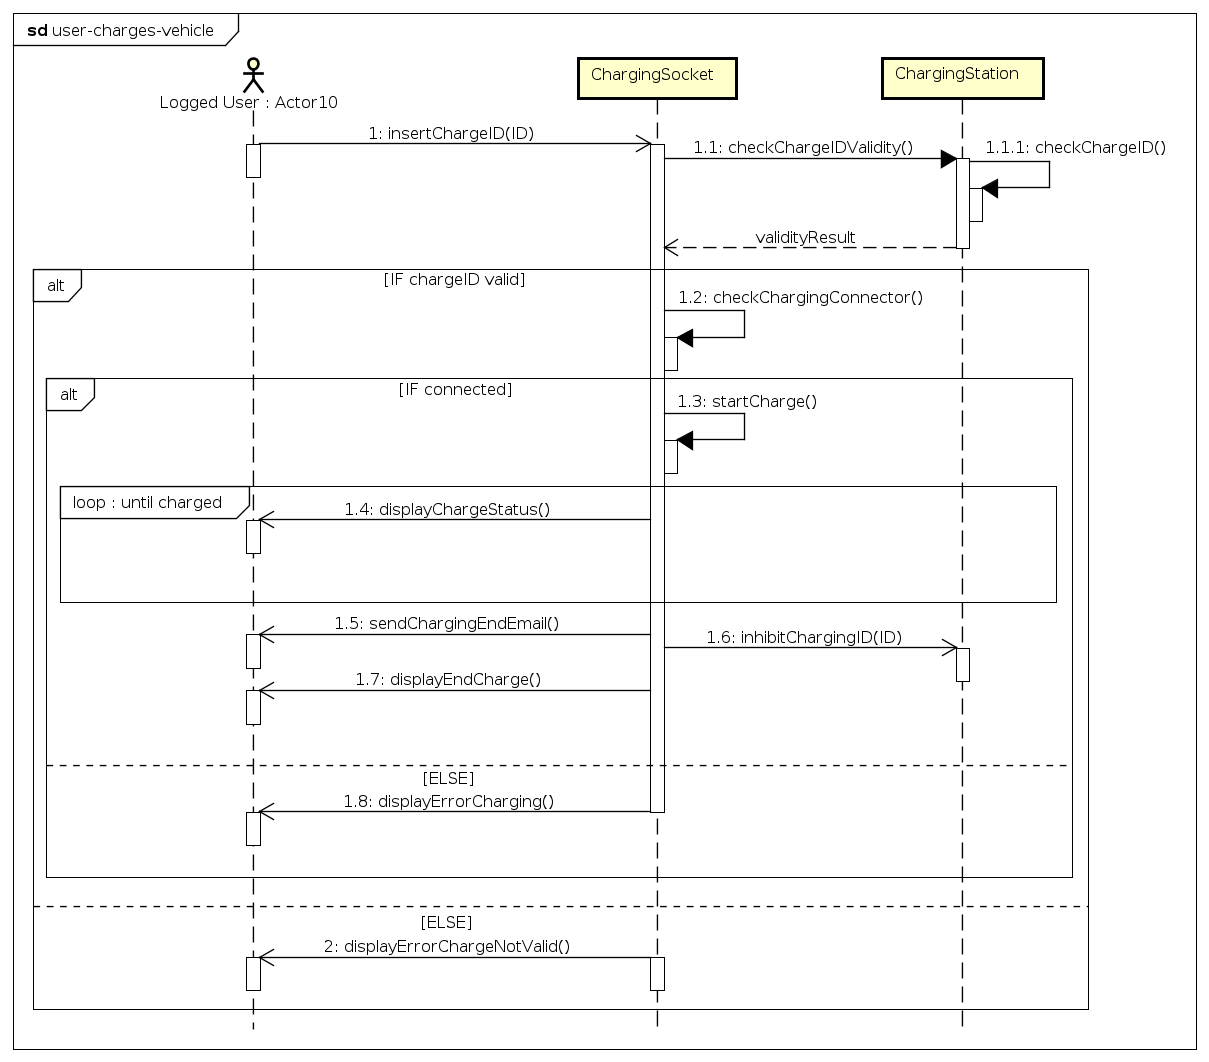
\includegraphics[keepaspectratio, width=16cm]{Sequence/user-charges-vehicle.png}
        \caption{Perform a charge sequence}
    \end{center}
\end{figure}
\begin{figure}[!h]
    \begin{center}
        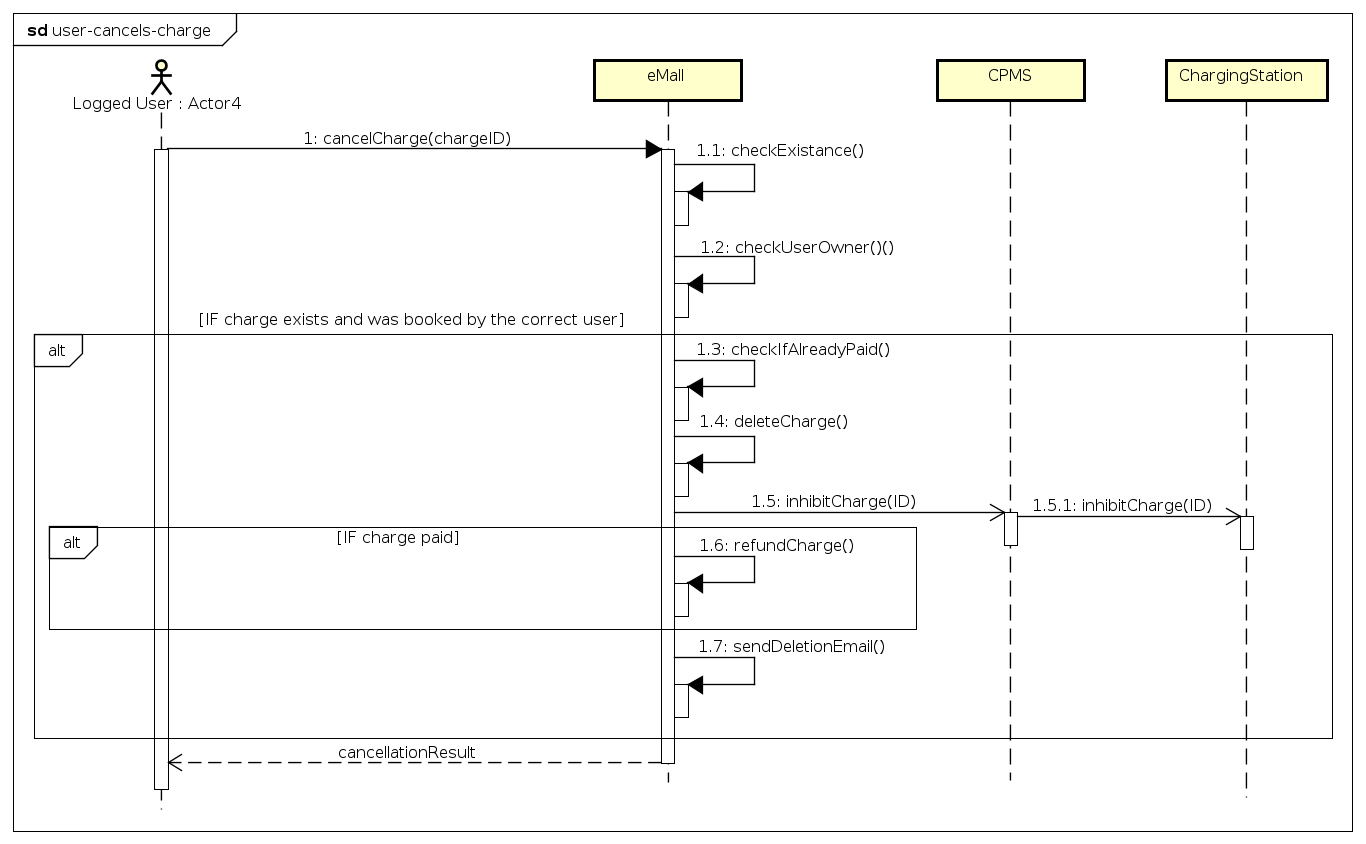
\includegraphics[keepaspectratio, width=16cm]{Sequence/user-cancels-charge.png}
        \caption{Cancel a charge sequence}
    \end{center}
\end{figure}
\begin{figure}[!h]
    \begin{center}
        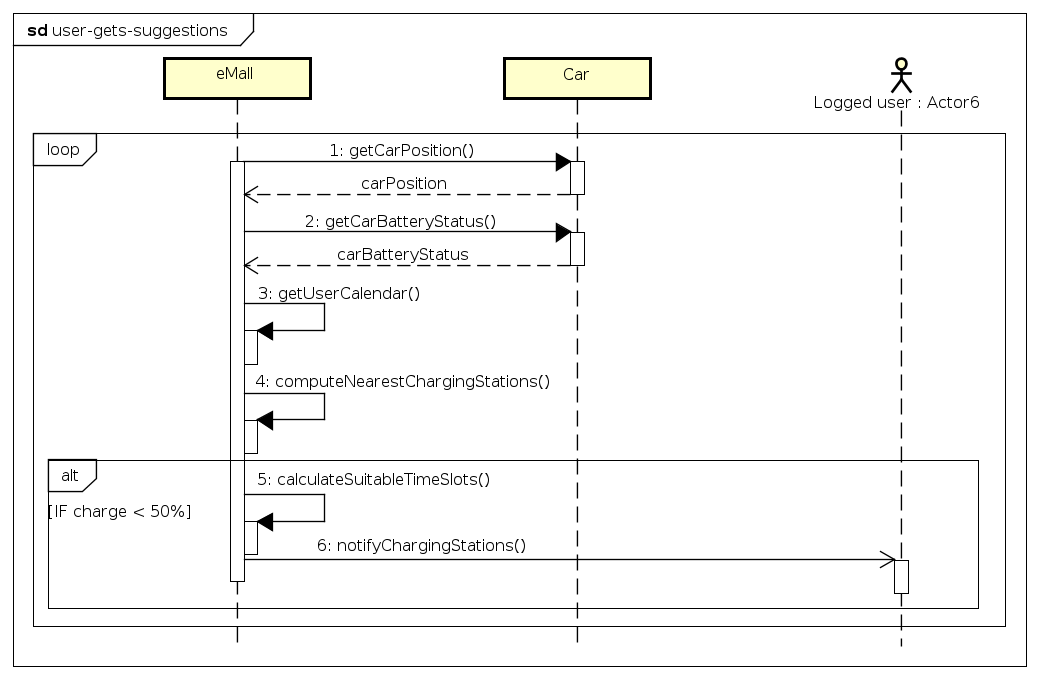
\includegraphics[keepaspectratio, width=16cm]{Sequence/user-gets-suggestions.png}
        \caption{Charging suggestions via calendar sequence}
    \end{center}
\end{figure}
\begin{figure}[!h]
    \begin{center}
        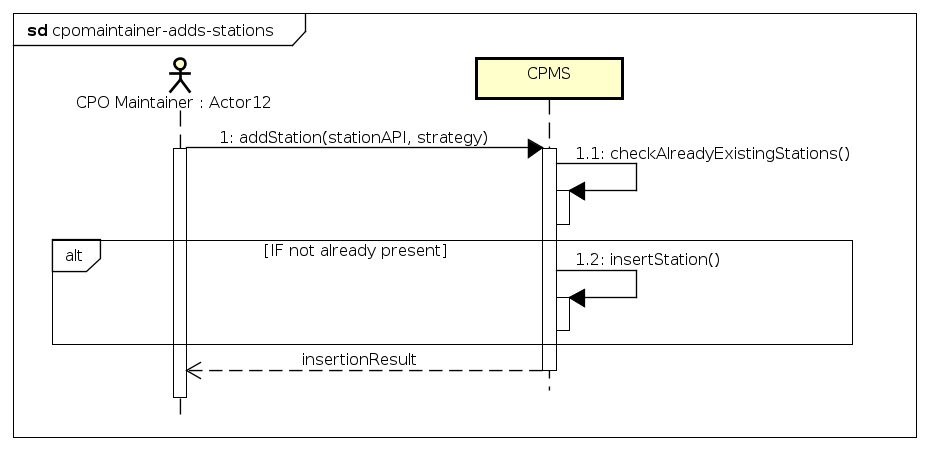
\includegraphics[keepaspectratio, width=16cm]{Sequence/cpomaintainer-adds-stations.png}
        \caption{\ac{CPO} maintainer adds stations to \ac{CPMS}}
    \end{center}
\end{figure}
\begin{figure}[!h]
    \begin{center}
        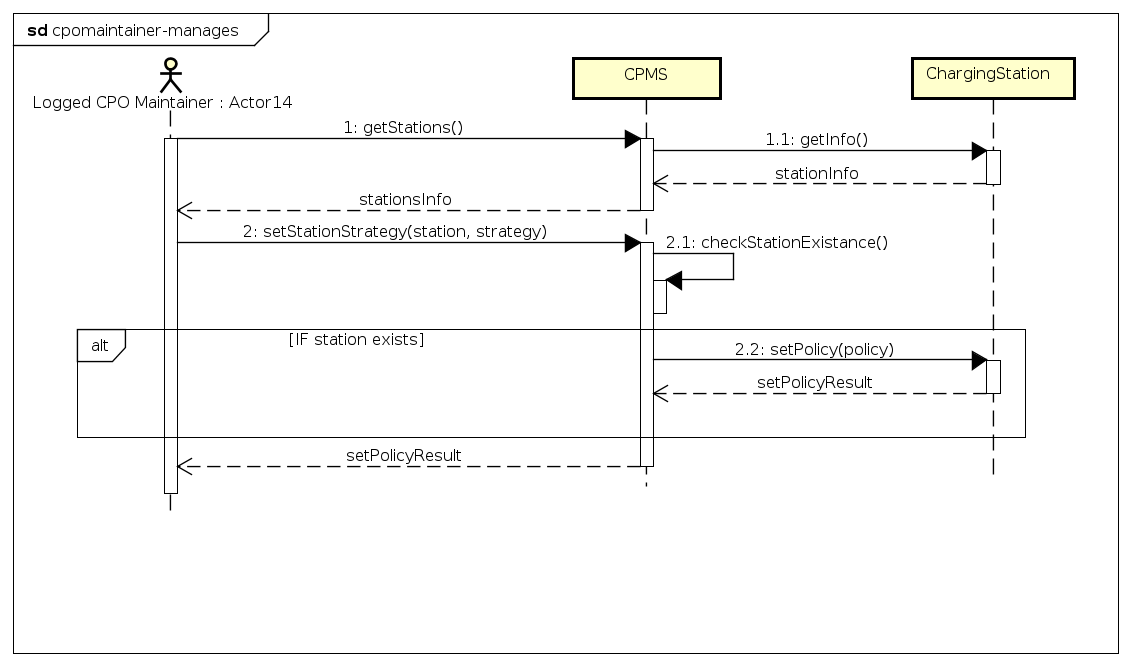
\includegraphics[keepaspectratio, width=16cm]{Sequence/cpomaintainer-manages.png}
        \caption{\ac{CPO} maintainer manages a \ac{CPMS}}
    \end{center}
\end{figure}

\clearpage
%Definition of use case diagrams, use cases and associated sequence/activity diagrams, and mapping on requirements
\subsection{Performance requirements}
The system in general needs to manage a large collection of electric car users/\acp{CPO} and it needs to supply the heaviest services (like computing the cheapest nearest stations) in a reasonable amount of time.
Because of that the system shall guarantee a baseline load of 1000000 users/\acp{CPO} still with a response time not greater than 5 seconds. To achieve the goal, the system shall be able to decentralize all the computation as much as possible,
trying to make the client responsible of the heaviest loads.
\subsection{Design constraints}
From this point we consider only the user side constraints as they represent the largest share of the system use base.
\subsubsection{Standards compliance}
The system must meet the following standards:
\begin{itemize}
    \item \textbf{\ac{GDPR} law}: The system must be compliant with the current GDPR law about users privacy;
    \item \textbf{Android and iOS}: The system must be compatible with the current versions and reasonably still used previous ones of Android and iOS.
\end{itemize}
\subsubsection{Hardware limitations}
Because the user side system consists of a smartphone app, the main hardware limitation is the computational capability of a smartphone processor. Hence the
application must be compatible with a low computational capability.

\subsection{Software system attributes}
\subsubsection{Reliability}
The system shall be fail safe, while the actual service can behave slower than expected it shall be still consistent with the results.
To do so the system shall be distributed data and performance wise, allowing a scalability factor while being open for maintenance without completely experiencing downtime.
Some good techniques are \ac{RACS} and \ac{RAPS} which put the reliability very high in the architecture.
\subsubsection{Availability}
Because a period of downtime would be detrimental, eMall has to prefer the availability over the conformity of response time.
Thus the availability should be as high as possible but greater than 99.99\% and must use some techniques to avoid down time during maintenance.
\subsubsection{Security}
Because the system will handle personal data, it has to abide the \ac{GDPR} law; thus an encryption of the user's password must be adopted and the access to the user's data must be restricted only to himself.
It is important that nobody else, not even the system administrator, can access the user's data in compliance of the privacy laws.\\
\subsubsection{Maintainability}
As stated in the Reliability and Availability sections, a good pattern for the whole system would be to consider the maintenance as less invasive as possible. Thus it would not be complicated to maintain a single or a restricted amount of nodes per time. This way the users would only experience at worst slowdowns but never downtime.
\subsubsection{Portability}
The system should be as cross platform as possible to increase the maintainability over different type of platforms.
\clearpage